% Chapter 1

\chapter{Deep Learning: Overview} % Main chapter title

\label{Chapter2} % For referencing the chapter elsewhere, use \ref{Chapter1} 

%----------------------------------------------------------------------------------------
% Define some commands to keep the formatting separated from the content 
%\newcommand{\keyword}[1]{\textbf{#1}}
%\newcommand{\tabhead}[1]{\textbf{#1}}
%\newcommand{\code}[1]{\texttt{#1}}
%\newcommand{\file}[1]{\texttt{\bfseries#1}}
%\newcommand{\option}[1]{\texttt{\itshape#1}}

In this chapter, we will provide a short overview of the theoretical concepts and recent advances in Deep Learning. We will give a basic introduction to neural networks, where we will discuss convolutional neural networks in more detail as these are the type of algorithms utilized in this work. We further will summarize some of the most popular convolutional neural network architectures.



%----------------------------------------------------------------------------------------

\section{Introduction to Deep Learning}

Deep Learning (DL) models have led to vast performance improvements in a large variety of domains, and therefore have gained substantial popularity over the last decade. These models were initially inspired by the human brain and analogies in neuroscience, which is why this class of algorithms is called neural networks (NN). The two most popular neural network architectures are convolutional neural networks (CNN) and recurrent neural networks (RNN). CNNs have driven major breakthroughs in visual object recognition \parencite{krizhevsky2012}, and image \parencite{zhang2015}, video \parencite{tompson2014} and audio \parencite{hinton2012} processing while RNNs brought about advances in research on sequential data, i.e. in speech and text \parencite{collobert2011}. However, the superior performance of Neural Networks compared to traditional machine learning algorithms is not limited to the aforementioned domains. Other fields in which NNs have advanced the state-of-the-art, for instance, include bioinformatics \parencite{junshui2015} and the analysis of data from elementary particle physics \parencite{ciodaroc2012}.


\textcolor{red}{CITE IN THIS SECTION}
Neural networks define a class of models that are composed of a variable number of processing layers (Hidden units) of simple models, and are generally used to map a fixed size input (e.g. the pixels of an image) to a fixed size output (e.g. a category or a probability). A Hidden unit of a fully connected neural network has connections between all the nodes of the previous layer and the next layer. These connections are fully parametrized by the weights of the network. In analogy to a firing neuron, a non-linear activation function is applied to the output of every Hidden unit. Historically, sigmoid and tanh have been used as activation functions. Nowadays the most popular activation function is the rectified linear unit (ReLU) $f(x) = max(0,x)$ \parencite{glorot2011}. We will see the reason for this at the end of the section. 
In Fig.~\ref{fig:simple_neural_net} we show an example of a fully connected 3-layer neural network. 

The strength of neural networks is that they can learn arbitrarily complex non-linear input-output mappings \parencite{cybenko1989}, and that they have the ability to automatically extract features from raw data. The latter is in stark cotrast to traditional machine learning algorithms, which require careful feature engineering. For instance, when dealing with images, the multi layer architecture of neural networks allows to learn different features at every stage of the network, where the complexity of the features increases as the network gets deeper.

\begin{figure}[h!]
	\centering
	\captionsetup{width=1\linewidth}
	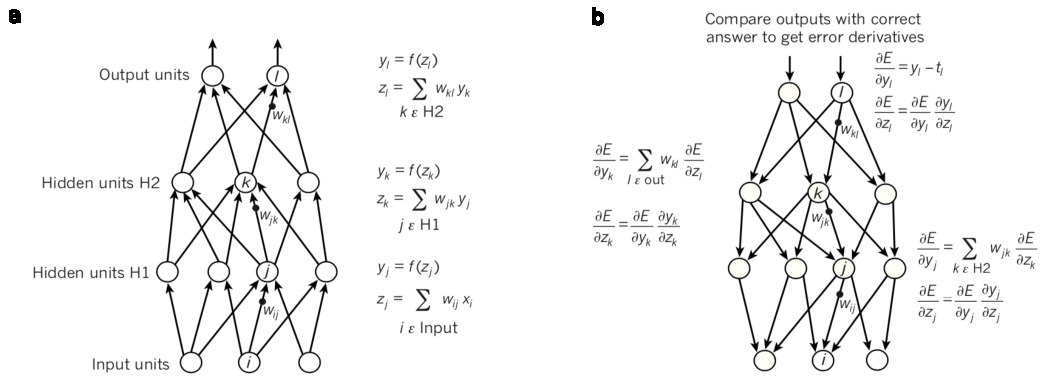
\includegraphics[width=1\textwidth]{Figures/simple_neural_net.pdf}
	\caption{\textbf{Example of 3-Layer Neural Network.} \textbf{(a)} Feed-forward representation of a neural network with two hidden units H1 and H2 and a binary output unit. The inputs to every layer are weighted averages, specified by the weights $w$, of the outputs of the previous layer. In every layer, the outputs are generated by applying a non-linear function to the inputs. The most popular function for this purpose is the ReLu (see text). \textbf{(b)} Back-propagation of the error in order to learn the optimal weights of the neural network. The error is quantified by a loss function $E$ at the output of the neural network, which is a measure of the discrepancy between the desired output and the actual output of the network. During backpropagation the chain-rule is applied recursively to the loss function in a backward manner. Specifically, at every layer the derivative of the error with respect to the inputs is computed by mutlipliying the upstream gradient with the local gradient. The upstream gradient is the derivative of the loss function with respect to the output of each unit, which is a weighted sum of the input derivatives of the layer above. The local gradient is the derivative of the non-linear function $f(z)$ with respect to its inputs. Starting from the output of the network one finally obtains the derivative of the loss function with respect to all weights, so that the network can minimze the loss by adjusting the weights. Panel is adapted from \parencite{lecun2015}.}
	\label{fig:simple_neural_net}
\end{figure}

ic gradient descent \parencite{bottou2008} or a variant of it. The computation of the gradient of the objective function with respect to all weights of the network is accomplished using backpropagation \parencite{rumelhart1986} (see Fig.~\ref{fig:simple_neural_net}(b)).
Intuitively,  {INTUITIVE EXPLANATION ABOUT BACKPROPAGATION}.


Althoug artifical neural networks have been known and studied since the 1950s, the first real breakthroughs were accomplished after the year 2009. The main reason for the specticism towards learning complex multilayer networks stemmed form the believe, that it was unfeasible to learn the parameters. However, in the last decade several many factors lead up to the explosion of deep learning and applications of which we will name some. First, with the advent of Big Data there suddenly there was enough data available to learn the hundreds of millions of parameters of a typical deep neural network. Second, the rectified linear unit solved the vanishsing gradient problem, so that much deeper networks could be trained. And last but not least, powerful graphics processing units (GPU) have turned out to be the ideal hardware to train large neural networks. All of these advances have led to the development of new network architectures, amongst one of them the convolutional neural networks.

\section{Convolutional Neural Networks}


\section{CNN Architectures}